\documentclass[11pt,a4paper]{article}
\usepackage[margin=24mm]{geometry}
\usepackage{amsmath,amssymb,amsthm,mathtools,booktabs,microtype}
\usepackage{tikz}
\usepackage[colorlinks=true,urlcolor=blue,citecolor=blue,linkcolor=blue]{hyperref}
\newtheorem{theorem}{Theorem}
\newtheorem{lemma}{Lemma}
\newtheorem{proposition}{Proposition}
\newcommand{\Z}{\mathbb Z}
\newcommand{\R}{\mathbb R}
\newcommand{\T}{\mathbb T}
\newcommand{\Dlt}{\Delta}
\newcommand{\e}{\mathrm e}
\title{\textbf{Exact Scalar Spectral Gaps and Topology-Selected Heat Covariances}\\on Compact Sol Manifolds}
\author{Tony Newton}
\date{}
\begin{document}
\maketitle
\begin{abstract}
For a canonically area-normalized family of compact hyperbolic torus bundles with Sol geometry, we prove an explicit trace-dependent spectral lower bound for every nonzero fiber Fourier sector, and identify the complete first positive scalar Laplace eigenvalue for monodromy traces three, four and five. The arithmetic input is a nonvanishing integral indefinite quadratic form conserved along each monodromy orbit; it reduces the scalar Laplacian exactly to confining one-dimensional Schrodinger operators. A harmonic-oscillator comparison excludes all fiber modes from the first eigenspace for these three traces. For a centered Gaussian scalar field with a prescribed Laplace heat covariance, we prove an exact Fourier-orbit selection rule, strict positivity within an orbit, and a covariance bound combining winding-distance Gaussian decay with the arithmetic spectral barrier. In a fixed canonical lattice basis, two selected modes correlate for trace three and are exactly uncorrelated for traces four and five. These are geometric scalar-field statements: no coupled Einstein--Boltzmann perturbation dynamics, CMB temperature/polarization prediction or observational discovery follows. Spectral arithmetic and quantum monodromy on Sol manifolds are established prior art; priority of the special explicit gap comparison is not established.
\end{abstract}

\section{Geometry, normalization, and scope}
For an integer $T\ge3$ define the hyperbolic unimodular matrix
\begin{equation}\label{eq:AT}
 A_T=\begin{pmatrix}T-1&T-2\\1&1\end{pmatrix},
 \quad D_T=T^2-4,\quad
 \lambda_T=\frac{T+\sqrt{D_T}}2,\quad
 k_T=\log\lambda_T=\operatorname{arcosh}(T/2)>0.
\end{equation}
Let
\[
P_T=
\begin{pmatrix}
\lambda_T-1&(\lambda_T^{-1}-1)/\sqrt{D_T}\\
1&1/\sqrt{D_T}
\end{pmatrix}.
\]
A direct computation gives $\det P_T=1$ and
$A_TP_T=P_T\operatorname{diag}(\lambda_T,\lambda_T^{-1})$.
On the universal cover $\R^2_x\times\R_w$ set $y=P_T^{-1}x$ and define
\begin{equation}\label{eq:metric}
g_T=dw^2+\e^{-2w}dy_1^2+\e^{2w}dy_2^2 .
\end{equation}
Take the quotient by $x\mapsto x+n$ for $n\in\Z^2$ and by
\[
(x,w)\mapsto(A_Tx,w+k_T).
\]
This is a compact torus bundle $M_T$ over a circle. The deck map acts
in the $y$-coordinates as
$(y_1,y_2,w)\mapsto(\lambda_Ty_1,\lambda_T^{-1}y_2,w+k_T)$,
which preserves \eqref{eq:metric}; the fiber translations also act
isometrically. Thus $g_T$ descends to $M_T$.
The determinant-one normalization makes $d\operatorname{vol}_{g_T}=d^2x\,dw$
and the $w$-circle has length $k_T$.

The displayed metric in $(y,w)$ is \emph{exactly the same local Sol
metric for every trace} $T$. Only its global identifications and
lattice-to-eigenframe maps differ. The question here concerns a
prescribed geometric scalar Laplacian and a Gaussian heat prior, not
a dynamically evolved cosmological perturbation. The classical
spectral separation of hyperbolic torus bundles and the relevant
indefinite quadratic forms were studied by Bolsinov, Dullin and
Veselov \cite{bdv}. The physical cosmic-topology covariance
programme in the COMPACT Collaboration concerns observables and
transfer functions well beyond this scalar model \cite{compact,overview}.

\section{An integral monodromy invariant and exact operator splitting}
\begin{lemma}[Nonzero integer orbit discriminant]\label{lem:q}
For $m=(m_1,m_2)\in\Z^2$, put
\begin{equation}\label{eq:Q}
Q_T(m):=\det(m,A_T^{\mathsf T}m)
=(T-2)m_1^2-(T-2)m_1m_2-m_2^2 .
\end{equation}
Then $Q_T(A_T^{\mathsf T}m)=Q_T(m)$.
For every nonzero integer $m$ one has $Q_T(m)\ne0$, hence
$|Q_T(m)|\ge1$. All nonzero dual-lattice orbits
$\{(A_T^{\mathsf T})^jm:j\in\Z\}$ are infinite.
\end{lemma}
\begin{proof}
The identity \eqref{eq:Q} follows by direct multiplication.
Since $\det A_T=1$,
\[
Q_T(A_T^{\mathsf T}m)
=\det(A_T^{\mathsf T}m,(A_T^{\mathsf T})^2m)
=\det(A_T^{\mathsf T})Q_T(m)=Q_T(m).
\]
The discriminant of the binary form is
$(T-2)^2+4(T-2)=T^2-4=D_T$, which lies strictly
between $(T-1)^2$ and $T^2$ for every integer $T\ge3$.
It is not a rational square. Were $Q_T(m)=0$
for a nonzero integer vector, the rational projective slope
of $m$ would be a root of this quadratic, a contradiction
(the cases $m_1=0$ and $m_2=0$ are also immediate).
Finally the two eigenvalues of every nonzero integer power of
$A_T^{\mathsf T}$ are $\lambda_T^{\pm j}\ne1$,
so no nonzero orbit can be periodic.
\end{proof}

Let $\alpha=P_T^{\mathsf T}m=(\alpha_1,\alpha_2)$.
The scalar Laplacian on the universal cover is
\[
-\Dlt_{g_T}=-\partial_w^2
-\e^{2w}\partial_{y_1}^2-\e^{-2w}\partial_{y_2}^2.
\]
Thus a fiber mode $\exp(2\pi i m\cdot x)$ is acted on by
\begin{equation}\label{eq:schrod}
H_m=-\frac{d^2}{dw^2}+V_m(w),\qquad
V_m(w)=4\pi^2\left(\alpha_1^2\e^{2w}
+\alpha_2^2\e^{-2w}\right).
\end{equation}
The explicit eigenvectors give the exact arithmetic identity
\begin{equation}\label{eq:product}
\alpha_1\alpha_2
=-\frac{Q_T(m)}{\sqrt{D_T}}.
\end{equation}
Hence both components of $\alpha$ are nonzero whenever
$m\in\Z^2\setminus\{0\}$, and the potential grows
exponentially toward both ends of $\R$. Each $H_m$ is a
confining self-adjoint Schrodinger operator with discrete spectrum.

\begin{lemma}[Unitary orbit decomposition]\label{lem:orbit}
For each nonzero dual-lattice orbit $\mathcal O(m)$, the scalar
$L^2(M_T)$ Fourier sector is unitarily equivalent to $L^2(\R,dw)$,
under which $-\Delta_{g_T}$ becomes $H_m$. The base Fourier
sector $m=0$ is the ordinary circle Laplacian
$-\partial_w^2$ on $\R/k_T\Z$.
\end{lemma}
\begin{proof}
The torus-bundle identification for an invariant scalar
$f$ is $f(A_Tx,w+k_T)=f(x,w)$. Writing
$f(x,w)=\sum_m f_m(w)\e^{2\pi im\cdot x}$ yields
\[
f_{A_T^{\mathsf T}m}(w)=f_m(w+k_T).
\]
Choose a representative $m$ of one orbit and define
$\psi(s)=f_m(s)$ on $\R$. Its complete Fourier orbit
is $f_{(A_T^{\mathsf T})^jm}(w)=\psi(w+jk_T)$.
Consequently
\[
\sum_{j\in\Z}\int_0^{k_T}
|f_{(A_T^{\mathsf T})^jm}(w)|^2dw
=\int_{\R}|\psi(s)|^2ds.
\]
The operator is compatible because
$V_{(A_T^{\mathsf T})^jm}(w)=V_m(w+jk_T)$.
For $m=0$, the deck condition is simply
$k_T$-periodicity in $w$.
\end{proof}

\section{A sharp trace-dependent potential inequality}
\begin{theorem}[All nonbase scalar modes: explicit spectral barrier]
\label{thm:barrier}
On the orthogonal complement of functions constant on each fiber,
\begin{equation}\label{eq:gapweak}
-\Dlt_{g_T}\ \ge\
\nu_T:=\frac{8\pi^2}{\sqrt{T^2-4}}
\end{equation}
as a quadratic-form inequality. In fact the stronger bound holds:
\begin{equation}\label{eq:gapstrong}
-\Dlt_{g_T}\ \ge\
\nu_T+\sqrt{2\nu_T}
=\frac{8\pi^2}{\sqrt{T^2-4}}
+\frac{4\pi}{(T^2-4)^{1/4}}
\end{equation}
on that subspace. These are rigorous lower bounds, not
claims that either quantity is an attained eigenvalue.
\end{theorem}
\begin{proof}
For $m\ne0$, \eqref{eq:product} and the arithmetic
nonvanishing lemma give
\[
V_m(w)\ge 8\pi^2|\alpha_1\alpha_2|
=\frac{8\pi^2|Q_T(m)|}{\sqrt{D_T}}
=:\mu_m\ge\nu_T.
\]
For the unique center $w_m=\tfrac12\log|\alpha_2/\alpha_1|$,
the potential can be written exactly as
$V_m(w)=\mu_m\cosh(2(w-w_m))$.
Since $\cosh(2s)\ge1+2s^2$ for all real $s$,
\[
H_m\ge-\partial_w^2+
\mu_m+2\mu_m(w-w_m)^2.
\]
The standard one-dimensional harmonic oscillator on the right
has ground energy $\mu_m+\sqrt{2\mu_m}$, which is increasing
in $\mu_m\ge\nu_T$.
Apply the unitary orbit decomposition
of Lemma~\ref{lem:orbit} and sum over all nonzero orbits.
\end{proof}

\section{Exact first positive eigenvalue for three trace controls}
The lower bound in Theorem~\ref{thm:barrier} can be combined
with a simple exact lower estimate for the deck length $k_T$.

\begin{theorem}[First scalar Laplace eigenvalue, $T=3,4,5$]
\label{thm:first}
For the metric \eqref{eq:metric}, if $T\in\{3,4,5\}$
the first positive eigenvalue of the entire scalar Laplacian is
\begin{equation}\label{eq:first}
\boxed{\quad
\lambda_1(M_T,g_T)
=\left(\frac{2\pi}{\log[(T+\sqrt{T^2-4})/2]}\right)^2 .
\quad}
\end{equation}
Its real eigenspace is exactly two-dimensional, spanned by
$\cos(2\pi w/k_T)$ and $\sin(2\pi w/k_T)$.
There is no nonzero fiber Fourier eigenfunction at or below this
eigenvalue. The trace restriction is essential to the proof below.
\end{theorem}
\begin{proof}
The base-circle eigenvalues are $(2\pi n/k_T)^2$,
$n\in\Z$, with first positive value $B_T=(2\pi/k_T)^2$.
We prove $B_T<\nu_T+\sqrt{2\nu_T}$ by strictly rational
inequalities.

Put $r_T=(T-2)/(T+2)\in(0,1)$.
The identity
\[
k_T=2\,\mathrm{artanh}(\sqrt{r_T})
=2\sum_{n=0}^{\infty}\frac{r_T^{n+1/2}}{2n+1}
>2\sqrt{r_T}\left(1+\frac{r_T}{3}\right)
\]
implies $B_T<C_T\pi^2$ with
\[
C_T=\frac{1}{r_T(1+r_T/3)^2}.
\]
In the table, choose upper rational bounds
$\sqrt{D_T}<s_T$ and $D_T^{1/4}<h_T$.
Then
$\nu_T+\sqrt{2\nu_T}>a_T\pi^2+b_T\pi$
where $a_T=8/s_T$, $b_T=4/h_T$.
Every entry in the final column is \emph{strictly positive}:
\[
\begin{array}{c|c|c|c|c}
T&C_T&a_T&b_T&
b_T-(C_T-a_T)\cdot(22/7)\\ \hline
3&1125/256&32/9&8/3&241/8064\\
4&243/100&16/7&2&3789/2450\\
5&343/192&8/5&16/9&12013/10080
\end{array}
\]
The radical upper bounds used here are, respectively,
$(s_T,h_T)=(9/4,3/2),(7/2,2),(5,9/4)$.
They are certified simply by squaring and taking fourth powers
of positive rational numbers.
Since $\pi<22/7$, the table shows
$C_T\pi^2<a_T\pi^2+b_T\pi$ in each of
the three cases. Theorem~\ref{thm:barrier} therefore excludes
the entire nonzero-fiber subspace at energy $B_T$.
The circle modes $n=\pm1$ attain $B_T$ and constitute
precisely the stated real eigenspace.
\end{proof}

\begin{table}[t]
\centering
\caption{Exact first spectral gap from Theorem~\ref{thm:first},
and a weaker general nonzero-fiber potential barrier. Entries
are shown numerically only as an aid to comparison; the proof is
exact and uses the rational table above.}
\begin{tabular}{ccccc}
\toprule
$T$ & $k_T$ & $\nu_T$ & $\nu_T+\sqrt{2\nu_T}$ & $\lambda_1$\\
\midrule
3 & $0.962424$ & $35.311$ & $43.714$ & $42.621$\\
4 & $1.316958$ & $22.793$ & $29.545$ & $22.762$\\
5 & $1.566799$ & $17.230$ & $23.100$ & $16.082$\\
\bottomrule
\end{tabular}
\label{tab:spectrum}
\end{table}

\section{Exact Gaussian heat-covariance selection}
Fix a trace $T\ge3$ and $\tau>0$. Let $X_T$ be a
centered real Gaussian scalar field on $M_T$ with prescribed
covariance
\[
C_{\tau,T}=\exp(-\tau[-\Delta_{g_T}]).
\]
This is a smooth positive trace-class covariance on the
compact manifold. Define the complex Fourier amplitudes of
its restriction to the section $w=0$ by
\[
F_m=\int_{\T^2}X_T(x,0)\e^{-2\pi i m\cdot x}\,d^2x.
\]
For $m\ne0$ write $m_j=(A_T^{\mathsf T})^j m$, and let
$K_m(s,s';\tau)$ denote the continuous integral kernel
of the positive Schrodinger heat semigroup $\e^{-\tau H_m}$
on $L^2(\R)$.

\begin{theorem}[Exact orbit mask and spectral heat bound]
\label{thm:cov}
For every nonzero $m,n\in\Z^2$,
\begin{equation}\label{eq:mask}
\mathbb E[F_m\overline{F_n}]=
\begin{cases}
K_m(0,jk_T;\tau)>0,
 &n=(A_T^{\mathsf T})^j m\quad(j\in\Z),\\
0,&n\notin\{(A_T^{\mathsf T})^j m:j\in\Z\}.
\end{cases}
\end{equation}
For modes $m_j,m_\ell$ on a common orbit,
the sharper coefficient-level statement is
\begin{equation}\label{eq:heat}
\boxed{\;
0<K_m(jk_T,\ell k_T;\tau)
\le \frac{\exp[-\mu_m\tau
-(j-\ell)^2k_T^2/(4\tau)]}{\sqrt{4\pi\tau}},
\qquad
\mu_m=\frac{8\pi^2|Q_T(m)|}{\sqrt{T^2-4}}.
\;}
\end{equation}
The upper bound holds for every $\tau>0$ and
is not an assertion that the covariance itself
is nonzero for arbitrary choices of a spectral prior.
\end{theorem}
\begin{proof}
Different nonzero $A_T^{\mathsf T}$-orbits define orthogonal
invariant subspaces of $-\Delta_{g_T}$ by
Lemma~\ref{lem:orbit}, and therefore also of its heat
covariance $C_{\tau,T}$. Their cross covariance vanishes.
On one orbit the unitary map of Lemma~\ref{lem:orbit}
identifies the two fiber coefficients at $w=0$ with
the evaluations of a one-dimensional field at
$s=jk_T$ and $s'=\ell k_T$. Its covariance kernel
is exactly $K_m(s,s';\tau)$, with no additional
volume factor because $\det P_T=1$.

By the Feynman--Kac Brownian-bridge representation
for $H_m=-\partial_s^2+V_m(s)$, the kernel
$K_m(s,s';\tau)$ is strictly positive at all
finite $s,s'$ and $\tau>0$. Indeed the free
Brownian-bridge kernel is positive, and the
exponential of the integral of the continuous
real confining potential is positive on every
continuous bridge path. The barrier
$V_m\ge\mu_m$ from \eqref{eq:product} bounds
that expectation by $\e^{-\tau\mu_m}$,
so
\[
0<K_m(s,s';\tau)\le
\frac{\e^{-\tau\mu_m}}{\sqrt{4\pi\tau}}\,
\e^{-(s-s')^2/(4\tau)}.
\]
Set $s=jk_T$, $s'=\ell k_T$ to obtain
\eqref{eq:heat}. The heat-kernel method is
standard \cite{feynman}, not a new physical
interaction law.
\end{proof}

A useful additional consequence of \eqref{eq:heat}
is the all-time exponential winding-distance envelope
\[
K_m(jk_T,\ell k_T;\tau)\le
\frac{1}{\sqrt{4\pi\tau}}\,
\exp\!\left[-|j-\ell|k_T\sqrt{\mu_m}\right],
\]
obtained by minimizing
$\mu_m\tau+(j-\ell)^2k_T^2/(4\tau)$
over positive $\tau$. The prefactor remains
$\tau$ dependent; this is not a uniform
time-independent pointwise bound.


\section{An exact trace-three / trace-four / trace-five contrast}
Consider the same two formal lattice labels in the
canonical integer basis for each bundle:
\[
m=(1,0),\qquad n=(2,1).
\]
From \eqref{eq:Q}, the arithmetic invariants are
\begin{equation}\label{eq:triplet}
\begin{array}{c|ccc}
T&Q_T(m)&Q_T(n)&\text{same orbit?}\\ \hline
3&1&1&\mathrm{yes}: n=A_3^{\mathsf T}m\\
4&2&3&\mathrm{no}\\
5&3&5&\mathrm{no}
\end{array}
\end{equation}
The no statements follow from unequal invariant
values; the yes statement is the explicit multiplication
$A_3^{\mathsf T}(1,0)=(2,1)$.
Theorem~\ref{thm:cov} therefore gives the
\emph{exact}, model-dependent contrast
\begin{equation}\label{eq:contrast}
\boxed{\quad
\mathbb E[F_{(1,0)}\overline{F_{(2,1)}}]
\begin{cases}
>0,&T=3,\\
=0,&T=4\text{ or }5,
\end{cases}
\qquad(\tau>0).
\quad}
\end{equation}
\begin{figure}[t]
\centering
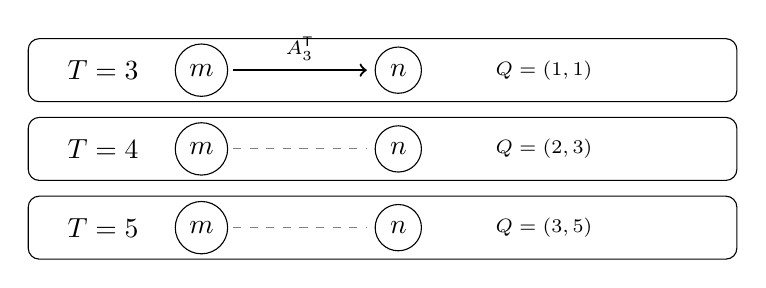
\begin{tikzpicture}
\node[draw,rounded corners,minimum width=9cm,
minimum height=0.8cm] at (0,2) {};
\node[draw,rounded corners,minimum width=9cm,
minimum height=0.8cm] at (0,1) {};
\node[draw,rounded corners,minimum width=9cm,
minimum height=0.8cm] at (0,0) {};
\node at (-3.55,2) {$T=3$};
\node at (-3.55,1) {$T=4$};
\node at (-3.55,0) {$T=5$};
\node[draw,circle] at (-2.3,2) {$m$};
\node[draw,circle] at (-2.3,1) {$m$};
\node[draw,circle] at (-2.3,0) {$m$};
\node[draw,circle] at (0.2,2) {$n$};
\node[draw,circle] at (0.2,1) {$n$};
\node[draw,circle] at (0.2,0) {$n$};
\draw[->,thick](-1.9,2)--(-0.2,2);
\node[above] at (-1.05,2) {\scriptsize $A_3^{\mathsf T}$};
\draw[dashed,gray](-1.9,1)--(-0.2,1);
\draw[dashed,gray](-1.9,0)--(-0.2,0);
\node at (2.05,2) {\scriptsize $Q=(1,1)$};
\node at (2.05,1) {\scriptsize $Q=(2,3)$};
\node at (2.05,0) {\scriptsize $Q=(3,5)$};
\end{tikzpicture}
\caption{Canonical-coordinate orbit selection for
$m=(1,0)$ and $n=(2,1)$. The solid arrow
represents a genuine deck Fourier link for $T=3$.
Dashed segments show no link at $T=4$ or $5$.}
\label{fig:selection}
\end{figure}

Equality of the conserved integer $Q_T$
is \emph{not sufficient} for orbit membership.
For instance
$Q_T(0,1)=Q_T(0,-1)=-1$ for every trace,
but no integer power of $A_T^{\mathsf T}$
takes a nonzero vector to its negative:
its eigenvalues are strictly positive.
The verification scripts therefore test
actual matrix powers, rather than
promoting an equality of $Q_T$
to an orbit-matching test.

The contrast \eqref{eq:contrast} is in a
\emph{chosen canonical lattice basis}.
An observer transformation or physical
radiation transfer map could change how
the relevant harmonics are represented.
Thus this is an exact property of the
specified scalar Gaussian heat prior,
not an observer-invariant CMB detection.

% PHY004_REMAINING
